\section{Software Architecture}

\frame{
 \begin{center}
  { \huge Software Architecture}
 \end{center}
}

\subsection{Overview}

\frame {
 \frametitle{Software Overview}
 \begin{itemize}
  \item Python on the backend
  \begin{enumerate}[A.]
   \item Django for the REST, HTTP stuff \cite{Web:Django}
   \item Custom python to interact with Arduino interface
  \end{enumerate}
  \item Heavy Javascript on the frontend
  \begin{enumerate}[A.]
   \item jqplot for creating graphs (jQuery included) \cite{Web:jQuery}
   \item django-compress to reduce the Javascript files to a manageable size.
   \item AngularJS for a MVC architecture that consumes the REST backend \cite{Web:AngularJS}
  \end{enumerate}
 \end{itemize}
}



\frame{
 \frametitle{Backend Overview}
 \begin{itemize}
  \item Django will be used to handle database
  \item Tastypie will be used to prototype the REST API
  \item Each functional area of the project is a Django module
  \begin{enumerate}[A.]
   \item System
   \item POW-R
   \item REST API
  \end{enumerate}
 \end{itemize}
}

\subsection{Architecture}

\frame{
 \frametitle{Backend Architecture}
 \begin{center}
  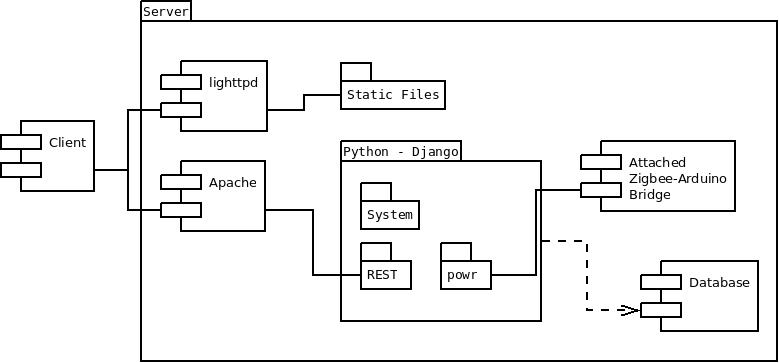
\includegraphics[width=0.8\textwidth]{Diagrams/ServerDependency.jpg}
 \end{center}
}

\frame{
 \frametitle{Frontend Architecture}
 \begin{itemize}
  \item django-compress
  \begin{enumerate}[A.]
   \item Minifies the JavaScript code so clients load faster
   \item Easy to use, can be tested
  \end{enumerate}
  \item AngularJS - MVC Architecture on the client-side
  \item jqplot - Renders charts and graphs
  \item jQuery - Deals with all the behind-the-scenes AJAX stuff
 \end{itemize}
}

\frame{
 \frametitle{Frontend Architecture}
 \begin{center}
  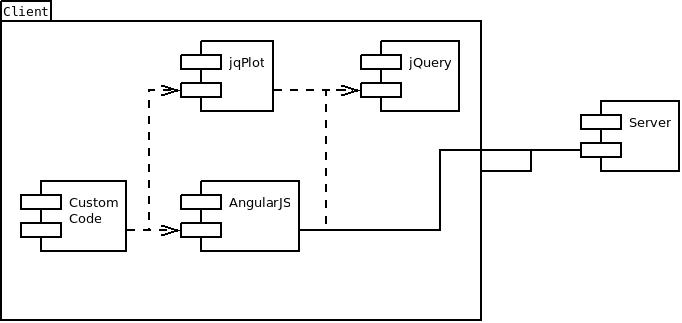
\includegraphics[width=0.8\textwidth]{Diagrams/ClientDependency.jpg}
 \end{center}
}